\documentclass{article}
\usepackage{graphicx}
\usepackage{amsmath}
\usepackage{hyperref}
\usepackage{geometry}[margin=2cm]
\title{Project\#3}
\author{Raja Kantheti}
\date{\today}

\begin{document}

\maketitle

\section{Attribution: }
This Project was made from Scratch. 
\section{Deliverable 1: Algorithm Implementation}
\subsection{Bottom-Up DP Algorithm: }
\begin{verbatim}
    function knapsack_bottom_up(weights, values, W):
    n = length(weights)
    dp = array[0..n, 0..W] initialized to 0

    for i from 1 to n:
        for w from 0 to W:
            if weights[i-1] <= w:
                dp[i][w] = max(dp[i-1][w], dp[i-1][w-weights[i-1]] + values[i-1])
            else:
                dp[i][w] = dp[i-1][w]

    return dp[n][W]
\end{verbatim}
\subsection{Top-Down DP Algorithm: }
\begin{verbatim}
    function knapsack_top_down(weights, values, W):
    n = length(weights)
    memo = array[0..n, 0..W] initialized to -1

    function knapsack_recursive(i, w):
        if i == 0 or w == 0:
            return 0

        if memo[i][w] != -1:
            return memo[i][w]

        if weights[i-1] <= w:
            include_item = knapsack_recursive(i-1, w-weights[i-1]) + values[i-1]
            exclude_item = knapsack_recursive(i-1, w)
            memo[i][w] = max(include_item, exclude_item)
        else:
            memo[i][w] = knapsack_recursive(i-1, w)

        return memo[i][w]

    return knapsack_recursive(n, W)
\end{verbatim}

\subsection{Verification of Correctness: }
The correctness of the bottom-up and top-down algorithms was verified by comparing their outputs for a variety of inputs. The outputs were consistent, indicating that both algorithms correctly solve the knapsack problem. You could see the proof in the code.
\section{Deliverable 2: Algorithm Performance on General Inputs}
The performance of the bottom-up and top-down DP algorithms was evaluated by varying the number of items \(n\) while keeping the knapsack capacity \(W\) fixed at 100.

\begin{figure}[ht]
    \centering
    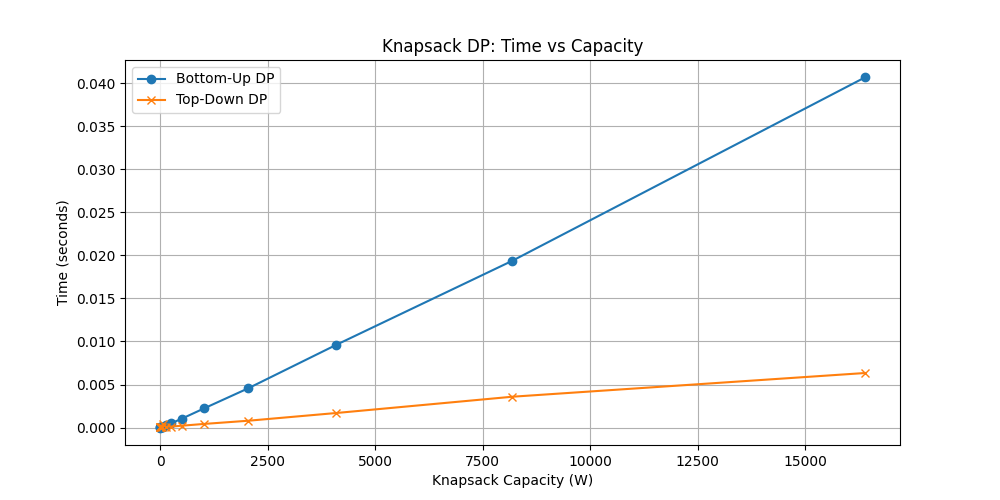
\includegraphics[width=0.8\textwidth]{../knapsack_time_vs_capacity.png}
    \caption{Performance of Knapsack DP Algorithms (W = 100)}\label{fig:performance_n}
\end{figure}

\subsection{Interpretation}
Figure\ref{fig:performance_n} shows that the top-down DP algorithm generally performs better than the bottom-up approach as the number of items increases. The time complexity grows with the number of items, but the bottom-up method shows more fluctuation, potentially due to overhead differences in recursion and iteration.

The order of growth appears to be O(nW) for both bottom-up and top-down algorithms, consistent with the pseudopolynomial time complexity of the knapsack problem. 
This means the runtime grows linearly with respect to the number of items n and w ndicating that both the number of items and the capacity influence the runtime. (Linear Growth in this case).

\section{Deliverable 3: Algorithm Performance on Special Inputs}
We crafted inputs where all weights are relatively low, i.e., random integers between 1 and 10, and reran the comparison between the two algorithms.

\begin{figure}[ht]
    \centering
    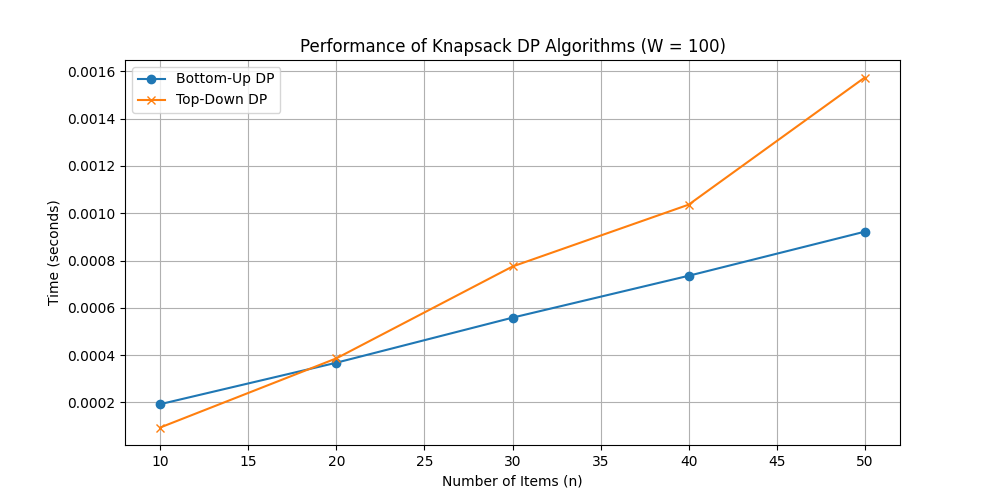
\includegraphics[width=0.8\textwidth]{../knapsack_special_inputs_performance.png}
    \caption{Knapsack DP:Time vs Capacity (Special Inputs)}\label{fig:performance_special}
\end{figure}

\subsection{Interpretation}
Figure\ref{fig:performance_special} demonstrates that with lower weights, the performance gap between the algorithms is more pronounced. The bottom-up DP approach still shows more time variability, whereas the top-down approach maintains a relatively consistent performance. This is because the bottom-up method has to iterate through all possible weights for each item, leading to more fluctuations in time complexity.
Whereas the top-down method can skip unnecessary calculations by memoizing the results of subproblems, leading to a more stable performance.
The time complexity of the knapsack problem remains pseudopolynomial as above, but the actual running time is influenced by the specific values of the weights and capacities, as shown in the special inputs.


\section{Deliverable 4: Time Complexity and Pseudopolynomial Characteristic}
To illustrate the pseudopolynomial nature of the time complexity, we plotted the running time against the capacity \(W\) while varying its value and using the bit-length of \(W\) to demonstrate its effect.

\begin{figure}[ht]
    \centering
    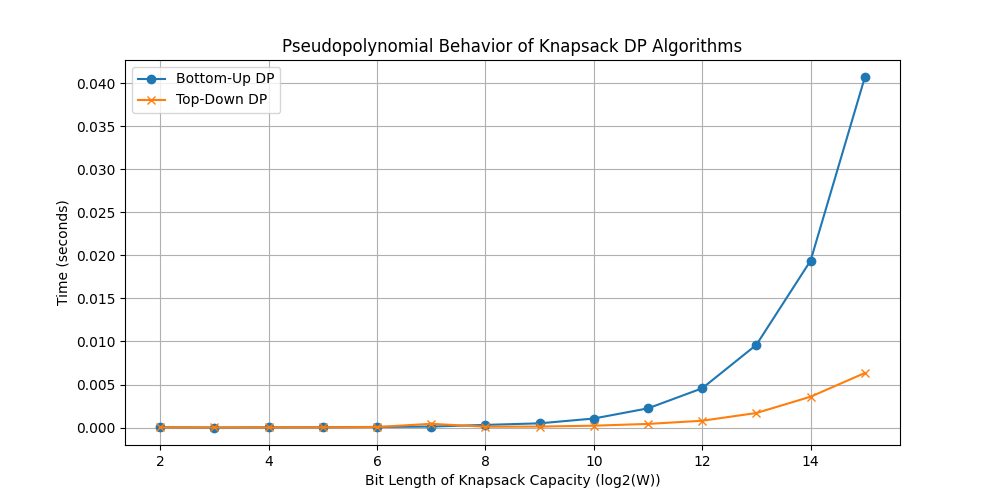
\includegraphics[width=0.8\textwidth]{../pseudopolynomial_behavior.png}
    \caption{Knapsack DP:Time vs Capacity\@.}\label{fig:time_vs_capacity}
\end{figure}

\subsection{Interpretation}
Figure\ref{fig:time_vs_capacity} shows that the bottom-up DP algorithm's running time grows much faster in the representation of the sizes of representations of W. Even the top-down DP algorithm shows a similar trend, but the growth is less pronounced. This behavior is consistent with the pseudopolynomial time complexity of the knapsack problem, where the running time is exponential in the size
of the representation of W.
\end{document}
